% This is text associated with the open textbook "Open Electromagnetics"
% See immediately below for author, date
% This work is licensed under the Creative Commons Attribution-ShareAlike 4.0 International License. (CC BY-SA 4.0) 
% To view a copy of the license, visit http://creativecommons.org/licenses/by-sa/4.0/

%ORB TITLE Propagation of a Uniform Plane Wave in an Arbitrary Direction
%ORB AUTHOR 0        # S.W. Ellingson, Virginia Tech (ellingson@vt.edu)
%ORB DATE 20191117   # yyyymmdd
%ORB ABSTRACT 

\label{m0165_Plane_Wave_Arbitrary_Direction} % <-- Must match name of this file and module directory name.  Don't mess with this!

An example of a uniform plane wave propagating in a lossless medium is shown in Figure~\ref{m0165_fEx}.
This wave is expressed in the indicated coordinate system as follows:
%
\begin{equation}
\widetilde{\bf E} = \hat{\bf x} E_0 e^{-j\beta z}
\label{m0165_eEx}
\end{equation}
%
\begin{figure}[b!] % <--- "[b]" for first figure in section *only*; delete for 2nd and subsequent figures
\begin{center}
\pdftooltip{{  % note double braces
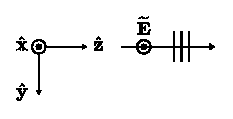
\includegraphics[width=2in]{modules/m0165_fEx.eps} 
% https://commons.wikimedia.org/wiki/File:Plane_wave_in_basic_coord.svg
}}{An x-y-z system with z hat horizontal, y hat vertical and pointing down, and x hat pointing out of the page. Capital E tilde out of page with plane wave traveling in the positive z direction.}
\end{center}
\centerline{\scriptsize 
\copyright~\hyperref[m0165_fEx_Credit]{C.\ Wang} 
\href{https://creativecommons.org/licenses/by-sa/4.0/}{CC BY-SA 4.0} 
} % \centerline 
\caption{
\label{m0165_fEx}
The plane wave described by Equation~\ref{m0165_eEx}.
}
\end{figure}
%
This is a phasor-domain expression for the electric field intensity, so $E_0$ is a complex-valued number representing the magnitude and reference phase 
\index{reference phase}
of the sinusoidally-varying wave.
The term ``reference phase'' is defined as the phase of $\widetilde{\bf E}$ at the origin of the coordinate system.
Since the phase propagation constant $\beta$ is real and positive, this wave is traveling in the $+\hat{\bf z}$ direction through simple lossless media.

Note that electric field intensity vector is linearly polarized in a direction parallel to $\hat{\bf x}$.
Depending on the position in space (and, for the physical time-domain waveform, time), $\widetilde{\bf E}$ points either in the $+\hat{\bf x}$ direction or the $-\hat{\bf x}$ direction. 
Let us be a bit more specific about the direction of the vector $\widetilde{\bf E}$.
To do this, let us define the \emph{reference polarization}
\index{reference polarization}
to be the direction in which $\widetilde{\bf E}$ points when $\mbox{Re}\left\{E_0 e^{-j\beta z}\right\}\ge 0$; i.e., when the phase of $\widetilde{\bf E}$ is between $-\pi/2$ and $+\pi/2$ radians.
Thus, the reference polarization of $\widetilde{\bf E}$ in Equation~\ref{m0165_eEx} is always $+\hat{\bf x}$.  

Note that Equation~\ref{m0165_eEx} indicates a specific combination of reference polarization and direction of propagation.
However, we may obtain any other combination of reference polarization and direction of propagation by rotation of the Cartesian coordinate system.
For example, if we rotate the $+x$ axis of the coordinate system into the position originally occupied by the $+y$ axis, then the very same wave is expressed as
%
\begin{equation}
\widetilde{\bf E} = -\hat{\bf y} E_0 e^{-j\beta z}
\label{m0165_eEy}
\end{equation}
%
This is illustrated in Figure~\ref{m0165_fEy}.
%
\begin{figure} % <--- "[b]" for first figure in section *only*; delete for 2nd and subsequent figures
\begin{center}
\pdftooltip{{  % note double braces
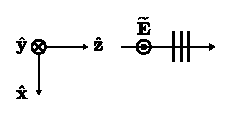
\includegraphics[width=2in]{modules/m0165_fEy.eps} 
% https://commons.wikimedia.org/wiki/File:Plane_wave_in_rotated_coord.svg
}}{An x-y-z system with z hat horizontal (right), x hat vertical and pointing down, and y hat pointing into the page. Capital E tilde out of page with plane wave traveling in the positive z direction.}
\end{center}
\centerline{\scriptsize 
\copyright~\hyperref[m0165_fEy_Credit]{C.\ Wang} 
\href{https://creativecommons.org/licenses/by-sa/4.0/}{CC BY-SA 4.0} 
} % \centerline 
\caption{
\label{m0165_fEy}
The same plane wave described in a rotated coordinate system, yielding Equation~\ref{m0165_eEy}.
}
\end{figure}
%
At first glance, it appears that the reference polarization has changed; however, this is due entirely to our choice of coordinate system.  
That is, the reference polarization is precisely the same; it is only the coordinate system used to describe the reference polarization that has changed.

Let us now rotate the $+z$ axis of the coordinate system around the $x$ axis into the position originally occupied by the $-z$ axis.
Now the very same wave is expressed as 
%
\begin{equation}
\widetilde{\bf E} = +\hat{\bf y} E_0 e^{+j\beta z}
\label{m0165_eEz}
\end{equation}
%
This is illustrated in Figure~\ref{m0165_fEz}.
%
\begin{figure} % <--- "[b]" for first figure in section *only*; delete for 2nd and subsequent figures
\begin{center}
\pdftooltip{{  % note double braces
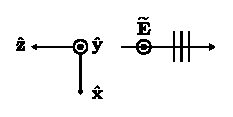
\includegraphics[width=2in]{modules/m0165_fEz.eps} 
% https://commons.wikimedia.org/wiki/File:Plane_wave_in_another_rotation_coord.svg
}}{An x-y-z system with z hat horizontal (left), x hat vertical and pointing down, and y hat pointing out of the page. Capital E tilde out of page with plane wave traveling in the negative z direction.}
\end{center}
\centerline{\scriptsize 
\copyright~\hyperref[m0165_fEz_Credit]{C.\ Wang} 
\href{https://creativecommons.org/licenses/by-sa/4.0/}{CC BY-SA 4.0} 
} % \centerline 
\caption{
\label{m0165_fEz}
The same plane wave described in yet another rotation of the coordinate system, yielding Equation~\ref{m0165_eEz}.
}
\end{figure}
%
At first glance, it appears that the direction of propagation has reversed; but, again, it is only the coordinate system that has changed, and not the direction of propagation.
Summarizing: Equations~\ref{m0165_eEx}, \ref{m0165_eEy}, and \ref{m0165_eEz} all represent the same wave.
They only appear to be different due to our choice for the orientation of the coordinate system in each case.

Now consider the same thought experiment for the infinite number of cases in which the wave does not propagate in one of the three basis directions of the Cartesian coordinate system.
One situation in which we face this complication is when the wave is obliquely incident on a surface.
In this case, it is impossible to select a single orientation of the coordinate system in which the directions of propagation, reference polarization, and surface normal can all be described in terms of one basis vector each.
To be clear:  There is no fundamental limitation imposed by this slipperiness of the coordinate system.  
However, practical problems such as the oblique-incidence scenario described above are much easier to analyze if we are able to express waves in a system of coordinates which always yields the same expressions.  

Fortunately, this is easily accomplished using \emph{ray-fixed coordinates}.
\index{ray-fixed coordinates}
Ray-fixed coordinates are a unique set of coordinates that are determined from the characteristics of the wave, as opposed to being determined arbitrarily and separately from the characteristics of the wave.
The ray-fixed representation of a uniform plane wave is:
%
\begin{equation}
\boxed{
\widetilde{\bf E}({\bf r}) = \hat{\bf e} E_0 e^{-j{\bf k}\cdot{\bf r}}
}
\label{m0165_eE}
\end{equation}
%
This is illustrated in Figure~\ref{m0165_fE}.
%
\begin{figure} % <--- "[b]" for first figure in section *only*; delete for 2nd and subsequent figures
\begin{center}
\pdftooltip{{  % note double braces
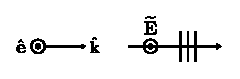
\includegraphics[width=2in]{modules/m0165_fE.eps} 
% https://commons.wikimedia.org/wiki/File:Plane_wave_in_ray-fixed_coord.svg
}}{Small e hat out of page in small k hat direction. Capital E tilde out of page with plane wave traveling in the k hat direction.}
\end{center}
\centerline{\scriptsize 
\copyright~\hyperref[m0165_fE_Credit]{C.\ Wang} 
\href{https://creativecommons.org/licenses/by-sa/4.0/}{CC BY-SA 4.0} 
} % \centerline 
\caption{
\label{m0165_fE}
A plane wave described in ray-fixed coordinates, yielding Equation~\ref{m0165_eE}.
}
\end{figure}
%
In this representation, 
${\bf r}$ is the position at which $\widetilde{\bf E}$ is evaluated, 
$\hat{\bf e}$ is the reference polarization expressed as a unit vector, and
${\bf k}$ is the unit vector $\hat{\bf k}$ in the direction of propagation, times $\beta$; i.e.:
%
\begin{equation}
{\bf k} \triangleq \hat{\bf k}\beta
\end{equation}
Consider Equation~\ref{m0165_eEx} as an example.
In this case, 
$\hat{\bf e}=\hat{\bf x}$,
${\bf k} = \hat{\bf z}\beta$, and (as always)
%
\begin{equation}
{\bf r} = \hat{\bf x}x +\hat{\bf y}y +\hat{\bf z}z
\end{equation}
%
Thus, ${\bf k}\cdot{\bf r}=\beta z$, as expected.

In ray-fixed coordinates, a wave can be represented by one -- and only one -- expression, which is the same expression regardless of the orientation of the ``global'' coordinate system.
Moreover, only two basis directions (namely, $\hat{\bf k}$ and $\hat{\bf e}$) must be defined.
Should a third coordinate be required, either $\hat{\bf k} \times \hat{\bf e}$ or $\hat{\bf e} \times \hat{\bf k}$ may be selected as the additional basis direction.
Note that the first choice has the possibly-useful feature that is the reference polarization of the magnetic field intensity $\widetilde{\bf H}$.

A general procedure for recasting the ray-fixed representation into a ``coordinate-bound'' representation is as follows.
First, we represent ${\bf k}$ in the new fixed coordinate system; e.g.:
%
\begin{equation}
{\bf k} = k_x\hat{\bf x} + k_y\hat{\bf y} + k_z\hat{\bf z} 
\end{equation}
%
where
%
\begin{flalign}
k_x &\triangleq \beta\hat{\bf k}\cdot\hat{\bf x} \\
k_y &\triangleq \beta\hat{\bf k}\cdot\hat{\bf y} \\
k_z &\triangleq \beta\hat{\bf k}\cdot\hat{\bf z}
\end{flalign}
%
Then,
%
\begin{equation}
{\bf k}\cdot{\bf r} = k_x x + k_y y + k_z z 
\end{equation}
%
With this expression in hand, Equation~\ref{m0165_eE} may be rewritten as:
%
\begin{equation}
\widetilde{\bf E} = \hat{\bf e} E_0 e^{-jk_x x} e^{-jk_y y} e^{-jk_z z} 
\end{equation}
%
If desired, one can similarly decompose $\hat{\bf e}$ into its Cartesian components as follows:
%
\begin{equation}
\hat{\bf e} = \left(\hat{\bf e}\cdot\hat{\bf x}\right)\hat{\bf x} 
        + \left(\hat{\bf e}\cdot\hat{\bf y}\right)\hat{\bf y} 
        + \left(\hat{\bf e}\cdot\hat{\bf z}\right)\hat{\bf z}  
\end{equation}
%
Thus, we see that the ray-fixed representation of Equation~\ref{m0165_eE} accommodates all possible combinations of direction of propagation and reference polarization.

%%%%%%%%%%%%%%%%%%%%%%%%%%%%%%%%%%%%%%%%%%%%%%%
%ORB EXAMPLE
~\\ \begin{example} 
\begin{mdframed}[backgroundcolor=brown!20,linecolor=brown!20]\raggedright
Plane wave propagating away from the $z$-axis.
\\~\\
A uniform plane wave exhibiting a reference polarization of $\hat{\bf z}$ propagates away from the $z$-axis.
Develop representations of this wave in ray-fixed and global Cartesian coordinates.

{\bf Solution}.
As always, the ray-fixed representation is given by Equation~\ref{m0165_eE}.
Since the reference polarization is $\hat{\bf z}$, $\hat{\bf e}=\hat{\bf z}$.
Propagating away from the $z$-axis means
%
\begin{equation}
\hat{\bf k} = \hat{\bf x}\cos\phi + \hat{\bf y}\sin\phi 
\end{equation}
%
where $\phi$ indicates the specific direction of propagation.
For example, 
$\phi=0$ yields $\hat{\bf k}=+\hat{\bf x}$,
$\phi=\pi/2$ yields $\hat{\bf k}=+\hat{\bf y}$,
and so on.
Therefore, 
%
\begin{equation}
{\bf k} \triangleq \beta\hat{\bf k} = \beta\left( \hat{\bf x}\cos\phi + \hat{\bf y}\sin\phi \right)  
\end{equation}
%
For completeness, note that the following factor appears in the phase-determining exponent in Equation~\ref{m0165_eE}: 
%
\begin{equation}
{\bf k}\cdot{\bf r} = \beta\left( x\cos\phi + y\sin\phi \right) 
\end{equation}
%
In this case, we see $k_x=\beta \cos\phi$, $k_y=\beta \sin\phi$, and $k_z=0$.
Thus, the wave may be expressed in Cartesian coordinates as follows:
%
\begin{equation}
\widetilde{\bf E} = \hat{\bf z} E_0 e^{-j\beta x \cos\phi} e^{-j\beta y \sin\phi} 
\end{equation}
%
\end{mdframed}
% note figures will need to go between "\end{mdframed}" and "\end{example}"
\end{example}
%%%%%%%%%%%%%%%%%%%%%%%%%%%%%%%%%%%%%%%%%%%%%%%




